\documentclass[12pt,a4paper]{article}

\renewcommand*\contentsname{Sadržaj}
\renewcommand{\figurename}{Slika}

\usepackage[margin=0.85in]{geometry}
\usepackage{graphicx}
\usepackage{float}
\usepackage{listings}
\usepackage{amsmath}

\renewcommand{\arraystretch}{1.5}
\begin{document}

\begin{titlepage}
	\centering
	{\scshape Univerzitet u Sarajevu \par}
	{\scshape Elektrotehnički Fakultet \par}
	\vspace{1cm}
	{\Large\scshape Prepoznavanje Oblika i Obrada Slike\par}
	\vspace{1.5cm}
	{\huge\bfseries Projektni Zadatak br. 1\par}
	\vspace{2cm}
	\Large Studenti: \par
	{\Large\itshape \textsc{Muftić} Belma, 1423/17260\par}
	{\Large\itshape \textsc{Lemeš} Lamija, 1474/17070\par}
	{\Large\itshape \textsc{Krupalija} Ehlimana, 1431/17461\par}
	\vfill
	Odgovorni asistent:\par
	MoE \textsc{Sumejja Porča}
	\vfill
	{\large Novembar, 2018\par}
\end{titlepage}

\pagenumbering{gobble}

\tableofcontents

\newpage

\pagenumbering{arabic}
\setcounter{page}{1}

\section{\textit{Dataset}}

\subsection{Tema projekta}

Projekat se bavi analizom fotografija različitih vrsta \textbf{krvnih ćelija}. Na slikama se nalaze četiri vrste krvnih ćelija:

\begin{enumerate}

\item \textit{Neutrophil};
\item \textit{Eosinophil};
\item \textit{Monocyte};
\item \textit{Lymphocyte}.

\end{enumerate}

Na slikama je potrebno pronaći ćeliju te odrediti kojoj od sljedećih klasa pripada:

\begin{enumerate}

\item \textit{Neutrophil};
\item \textit{Lymphocyte};
\item Ništa od navedenog (neka druga vrsta krvne ćelije).

\end{enumerate}

Nakon toga potrebno je izdvojiti ćeliju i označiti njenu poziciju na slici.

\subsection{Opis \textit{dataset}-a}

\textit{Dataset} se sastoji od \textbf{12,444} slika. Među tim slikama nalaze se četiri prethodno opisane klase (odnosno vrste krvnih ćelija). Broj uzoraka svake klase prikazan je u sljedećoj tabeli: \\

\begin{center}
\def\arraystretch{1.5}%
\begin{tabular}{| p{3cm} | p{3cm} | p{3cm} | p{3cm} |} \hline

\textbf{Klasa} 						& \textbf{Uzorci za trening}			& \textbf{Uzorci za testiranje}			& \textbf{Ukupan broj uzoraka} 	\\ \hline
\textit{Neutrophil} 					& 2,499								& 624								& 3,123	  						\\ \hline
\textit{Eosinophil} 					& 2,497								& 623								& 3,120	  						\\ \hline
\textit{Monocyte} 					& 2,478								& 620								& 3,098	  						\\ \hline
\textit{Lymphocyte} 					& 2,483								& 620								& 3,103	  						\\ \hline

\end{tabular}
\end{center}

~\\

Za svrhe ovog projekta biti će upotrijebljeno ukupno \textbf{90 slika} (po \textbf{30 slika} za sve tri klase: \textit{Neutrophils}, \textit{Lymhocythes}, ostalo).

\newpage

\section{\textit{DataPrep2}}

\subsection{Uklanjanje šuma}

Za uklanjanje šuma (zamagljivanje slike - \textit{blurring}) izvršen je izbor između sljedećih filtera:

\begin{itemize}

\item \textbf{Filter na bazi prosjeka (\textit{Averaging filter}):} Vrijednost piksela mijenja se sa srednjom vrijednošću svih piksela u oblasti od interesa (na ovaj način zamagljenje slike bude veoma veliko); 
\item \textbf{Filter na bazi statističkog prosjeka (\textit{Mediana filter}):} Vrijednost piksela mijenja se sa medijanom uzorka (efekat zamagljenja je manji);
\item \textbf{Bilateralni filter:} Pri računanju vrijednosti za zamjenu vrši se računanje prosjeka samo za okolinu nekog piksela, što ne uključuje cijelu oblast od interesa (kao rezultat, ivice će biti očuvane, odnosno neće biti zamagljene, dok će se šum smanjiti u ostalim dijelovima slike)

\end{itemize}

Za upotrebu je odabran \textbf{bilateralni filter}, jer iako je sporiji od ostalih filtera, ne zamagljuje ivice, čije je očuvanje važno pri analizi krvnih ćelija. \\

Na sljedećoj slici prikazan je prije i nakon vršenja redukcije šuma korištenjem bilateralnog filtera:

\begin{figure}[H]

\center
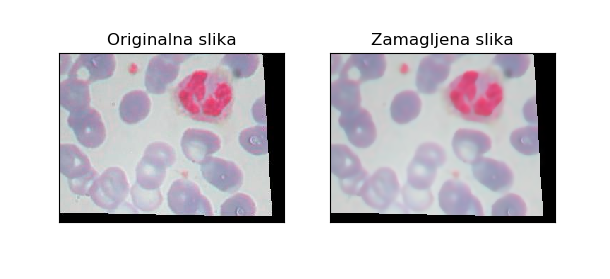
\includegraphics[scale=0.9]{s1SmanjenjeSuma.png}
\caption{Smanjenje šuma na slici korištenjem bilateralnog filtera}

\end{figure}

\subsection{Maskiranje neoštrina}

Za maskiranje neoštrina izabrana je kernel matrica sa vrijednostima:
\[
\begin{bmatrix}
    0 & -2 & 0 \\
    -2 & 9 & -2 \\
    0 & -2 & 0
\end{bmatrix}
\]

Na slici ispod prikazan je rezultat izoštravanja u odnosu na originalnu sliku:


\begin{figure}[H]

	\center
	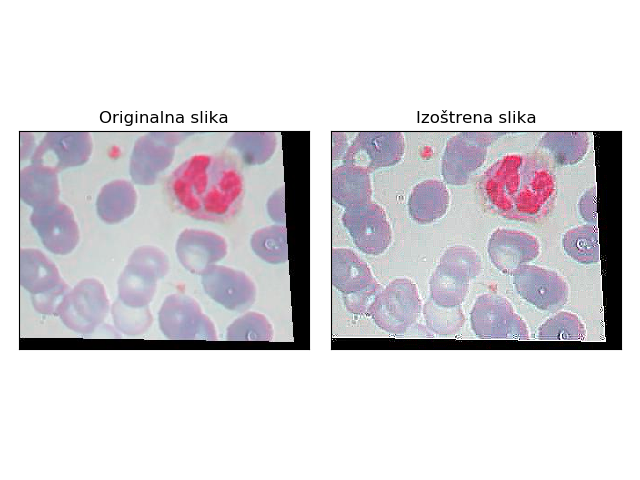
\includegraphics[scale=0.9]{s2MaskiranjeNeostrina.png}
	\caption{Smanjenje šuma na slici korištenjem filtera za maskiranje neoštrina}
	
\end{figure}

\newpage

\section{\textit{DataPrep3}}

\subsection{Poboljšavanje kvaliteta slika}

\subsection{Poboljšavanje kontrasta}

Za poboljšavanje kontrasta slike korištena su tri različita postupka, koji će biti opisani u nastavku.

\subsubsection{Aritmetičke operacije}

Kako bi se poboljšao kontrast slike, prvenstveno je neophodno pretvoriti RGB u HLS sliku. Zatim se vrši manipulacija nad pikselima koji označavaju \textit{Luminence} u okviru tako transformisane slike. Koriste se aritmetičke operacije nad pojedinačnim pikselima slike, na sljedeći način:

\begin{itemize}

\item Ukoliko je vrijednost piksela manja od srednje vrijednosti svih \textit{Luminence} piksela, vrši se \textbf{smanjenje vrijednosti piksela} za iznos faktora koji se može prilagođavati (svijetli pikseli postaju svjetliji za iznos faktora);
\item Ukoliko je vrijednost piksela veća od srednje vrijednosti svih \textit{Luminence} piksela, vrši se \textbf{povećanje vrijednosti piksela} za iznos faktora koji se može prilagođavati (tamni pikseli postaju tamniji za iznos faktora).

\end{itemize}

Na sljedećoj slici prikazan je izgled slike prije i nakon vršenja poboljšanja za vrijednost faktora \texttt{factor = 30}:

\begin{figure}[H]

\center
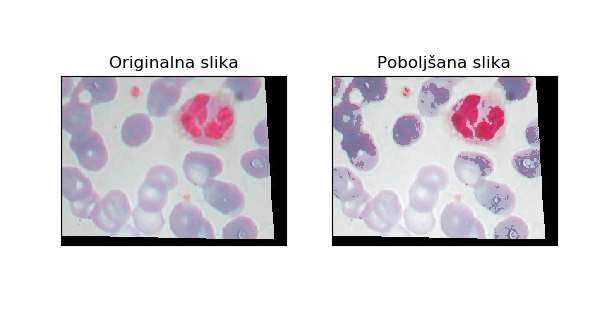
\includegraphics[scale=0.9]{s3Kontrast1.png}
\caption{Poboljšavanje kontrasta slike korištenjem aritmetičkih operacija}

\end{figure}

\subsubsection{Linearno razvlačenje kontrasta}

Drugi metod poboljšanja kontrasta slike postiže se manipulacijom nad pojedinačnim kanalima slike. Svaka vrijednost piksela se određuje u zavisnosti od vrijednosti susjednih piksela. Intenzitet se izračunava pomoću formule za normalizaciju:
\[
	I_o = (I_i - Min_i) * (((Max_o - Min_o) / (Max_i - Min_i)) + Min_o)
\]

Gdje su vrijednosti:

\begin{itemize}
\item I\textsubscript{o} - Izlazna vrijednost piksela
\item I\textsubscript{i} - Ulazna vrijednost piksela
\item Min\textsubscript{i} - Minimalna vrijednost piksela u ulaznoj slici
\item Max\textsubscript{i} - Maksimalna vrijednost piksela u ulaznoj slici
\item Min\textsubscript{o} - Minimalna vrijednost piksela u izlaznoj slici
\item Max\textsubscript{o} - Maksimalna vrijednost piksela u izlaznoj slici
\end{itemize}

Na sljedećoj slici prikazan je izgled slike prije i nakon linearnog razvlačenja kontrasta:

\begin{figure}[H]

	\center
	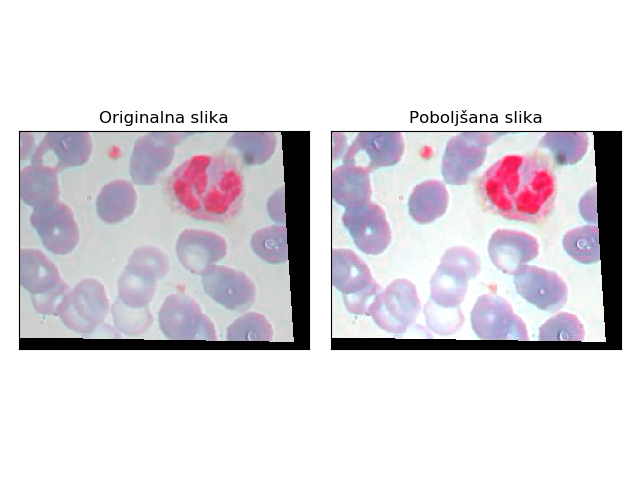
\includegraphics[scale=0.9]{s3Kontrast2.png}
	\caption{Poboljšavanje kontrasta slike korištenjem linearnog razvlačenja}
	
\end{figure}

\subsection{Povećanje osvjetljenja}

Za povećanje osvjetljenja slike korištena su tri različita postupka, koji će biti opisani u nastavku.

\subsubsection{Aritmetičke operacije}

Kako bi se povećalo osvjetljenje slike, prvenstveno je neophodno pretvoriti RGB u HLS sliku. Zatim se vrši manipulacija nad pikselima koji označavaju \textit{Luminence} u okviru tako transformisane slike. Koristi se aritmetička operacija \textbf{sabiranja} pojedinačnih piksela slike sa iznosom faktora (koji se može prilagođavati).


Na sljedećoj slici prikazan je izgled slike prije i nakon vršenja poboljšanja za vrijednost faktora \texttt{factor = 30}:

\begin{figure}[H]

\center
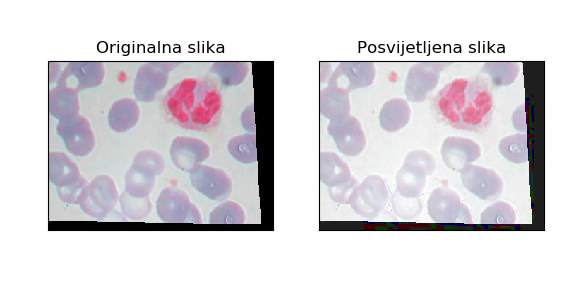
\includegraphics[scale=0.9]{s6Osvjetljenje1.png}
\caption{Povećanje osvjetljenja slike korištenjem aritmetičke operacije sabiranja}

\end{figure}

\subsubsection{Linearne transformacije}

Drugi metod za povećanje osvjetljenja slike podrazumijeva primjenu linearnih transformacija. Konkretno promjena vrijednosti parametra beta u OpenCV funkciji \textit{convertScaleAbs}.

Na sljedećoj slici je izgled slike prije i nakon povećanja osvjetljenja postavljanjem vrijednosti parametra beta na 20 (moguće su vrijednosti od 0 do 100):

\begin{figure}[H]

	\center
	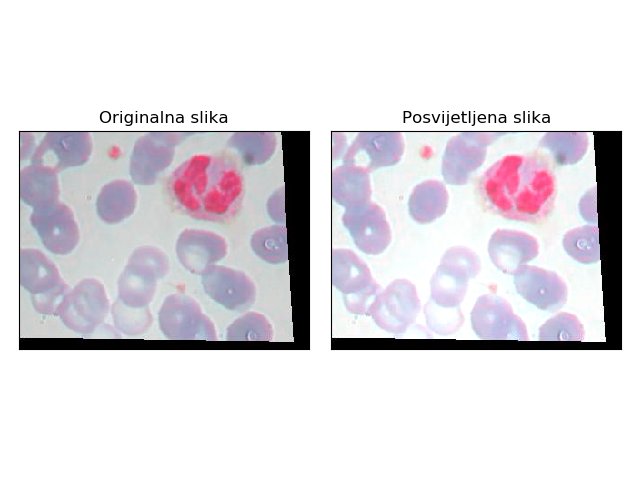
\includegraphics[scale=0.9]{s6Osvjetljenje2.png}
	\caption{Povećanje osvjetljenja slike korištenjem linearne transformacije}
	
\end{figure}

\subsection{Ujednačavanje histograma}

Za ujednačavanje histograma slike korištena su tri različita postupka, koji će biti opisani u nastavku.

\subsubsection{Raspodjela vjerovatnoća}

Kako bi se ujednačio histogram slike, prvenstveno je neophodno pretvoriti RGB u HLS sliku. Zatim se vrši analiza piksela koji označavaju \textit{Luminence} u okviru tako transformisane slike. Za svaki piksel pronalazi se njegova okolina (čija veličina ovisi o iznosu prilagodljivog faktora), te se zatim pronalazi vrijednost \textbf{piksela s najmanjom frekvencijom pojavljivanja} iz te okoline. Zatim se trenutni piksel izjednačava s tom vrijednošću i vrijednost frekvencije piksela povećava. Na ovaj način postiže se ujednačavanje histograma, odnosno preraspodjela vjerovatnoće pojavljivanja piksela u okolinu. \\

Na sljedećoj slici prikazan je izgled slike i njenog pripadajućeg histograma prije i nakon vršenja ujednačavanja histograma za vrijednost faktora \texttt{factor = 30}:

\begin{figure}[H]

\center
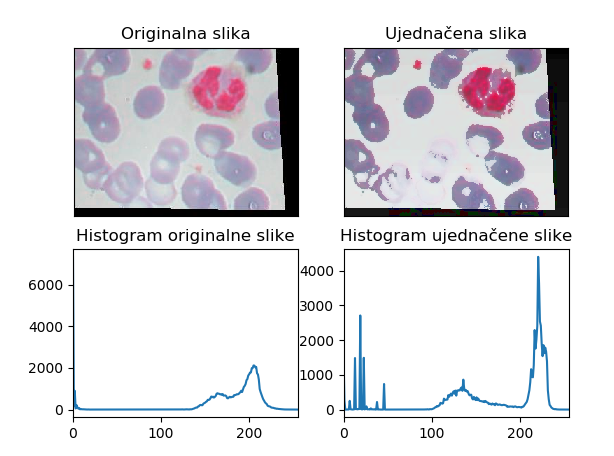
\includegraphics[scale=0.9]{s9Histogram1.png}
\caption{Ujednačavanje histograma slike korištenjem raspodjele vjerovatnoća}

\end{figure}

\subsubsection{CLAHE}

Drugi metod ujednačavanja histograma slike jeste CLAHE (eng. \textit{Contrast Limited Adaptive Histogram Equalization}). Da bi se omogućilo korištenje ovog tipa ujednačavanja, sliku je bilo potrebno prethodno pretvoriti u \textit{grayscale}.

Na sljedećoj slici prikazan je izgled slike i njenog histograma prije i nakon izvršenja ujednačavanja histograma za vrijednost faktora \texttt{factor = 10}:

\begin{figure}[H]

	\center
	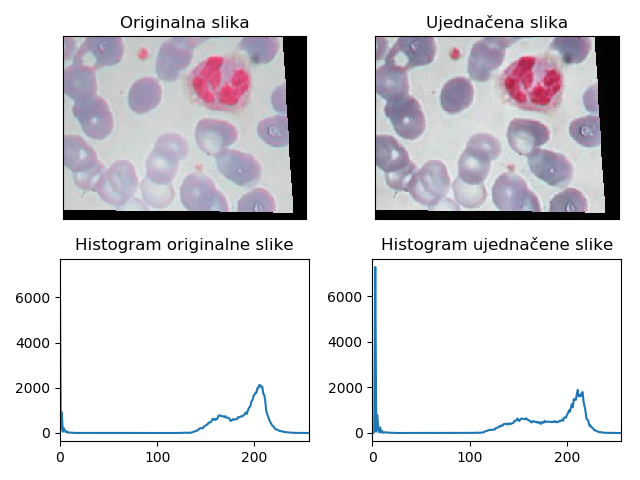
\includegraphics[scale=0.9]{s9Histogram2.png}
	\caption{Ujednačavanje histograma slike korištenjem CLAHE}
	
\end{figure}

\end{document}